\documentclass{standalone}
\usepackage{graphicx}
\usepackage{enumitem}
\usepackage{subcaption}
\usepackage{tikz}

\begin{document}
\begin{tikzpicture}
    % First figure
    \node[draw, rectangle, blue] (figure1) at (0,0) {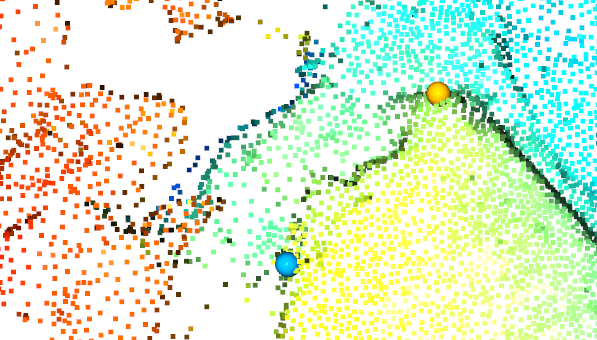
\includegraphics[width=0.3\textwidth]{reference.png}};
    \node[above=50pt, text width=3cm,align=center] at (figure1) {Known size reference};

    % Second figure
    \node[draw, rectangle, blue] (figure2) at (4,0) {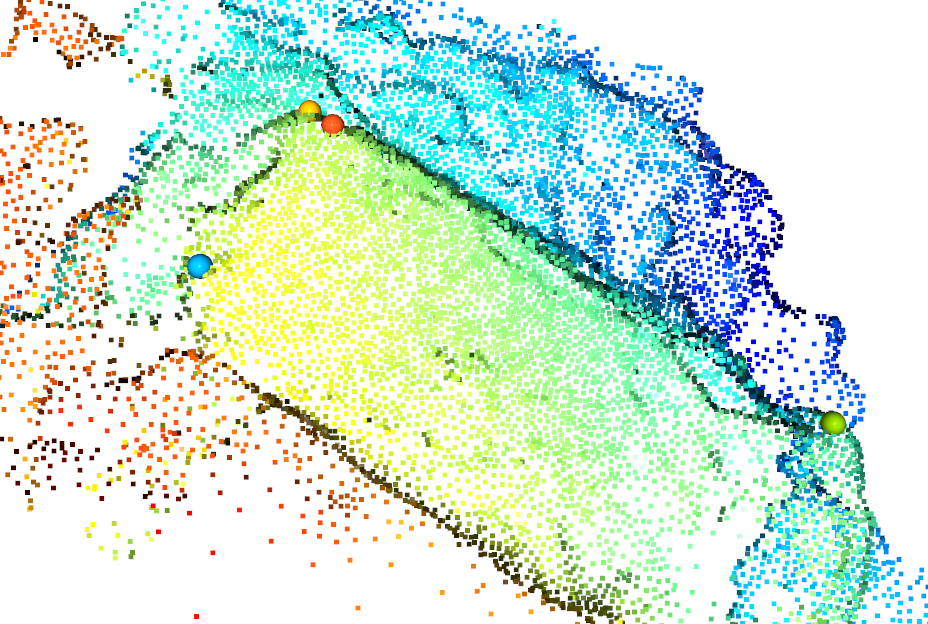
\includegraphics[width=0.25\textwidth]{distance to be measured.png}};
    \node[above=50pt, text width=50pt,align=center] at (figure2) {Distance to be measured};

    % Third figure
    \node[draw, rectangle, blue] (figure3) at (8,0) {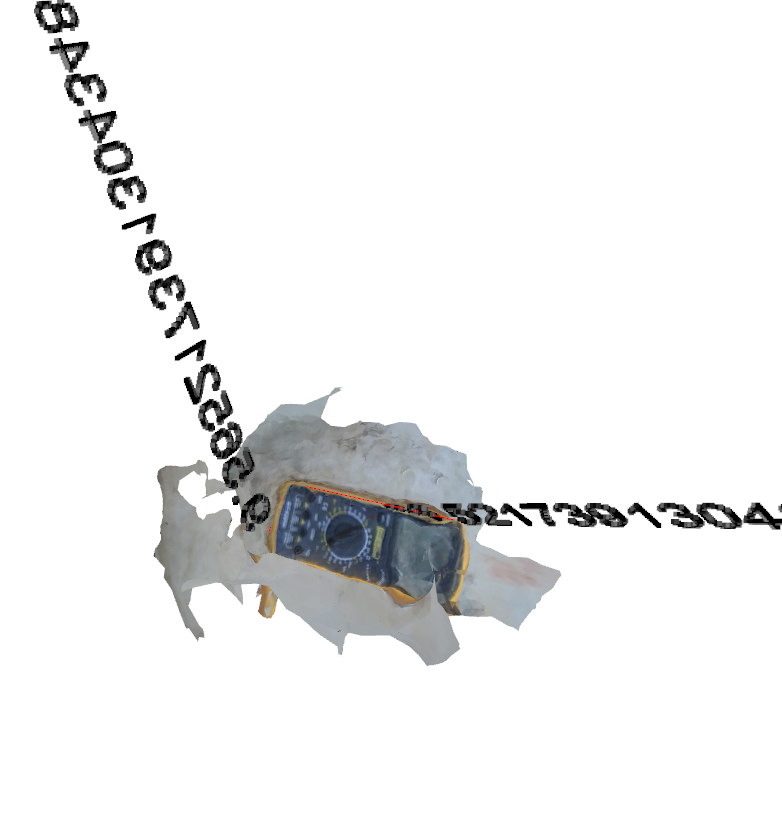
\includegraphics[width=0.27\textwidth]{output distances.png}};
    \node[above=70pt,text width=50pt,align=center] at (figure3) {Measured distance};

    % Arrow between figures
    \draw[->, line width=1.3pt, blue] (figure1) -- (figure2);
    \draw[->, line width=1.3pt, blue] (figure2) -- (figure3);

\end{tikzpicture}
\end{document}